\documentclass[10pt]{beamer}

\usetheme{metropolis}
\usepackage{appendixnumberbeamer}

\usepackage{booktabs}
\usepackage[scale=2]{ccicons}

\usepackage{pgfplots}
\usepgfplotslibrary{dateplot}

\usepackage{xspace}
\newcommand{\themename}{\textbf{\textsc{metropolis}}\xspace}

\usepackage[spanish]{babel}

\title{React}
\subtitle{Una biblioteca en Javascript para crear interfaces}
\date{\today}
\author{Betology}
\institute{Amor, comprensión y ternura}

\begin{document}

\maketitle

\begin{frame}{Tabla de contenidos}
  \setbeamertemplate{section in toc}[sections numbered]
  \tableofcontents[hideallsubsections]
\end{frame}

% Sección 1: ¿Qué es React?
\section{¿Qué es React?}

\begin{frame}

  \begin{itemize}
    \item Biblioteca de JavaScript para construir interfaces de usuario.
    \item Desarrollada por Facebook.
    \item Utiliza componentes para construir interfaces modulares y reutilizables.
  \end{itemize}
\end{frame}

% Sección 2: Componentes de React
\section{Componentes de React}

% Diapositiva 1: Definición de un Componente
\begin{frame}[fragile]
  \frametitle{Definición de un Componente}
  \begin{itemize}
    \item Los componentes son bloques de construcción en React.
    \item Pueden ser definidos como clases o funciones.
  \end{itemize}
    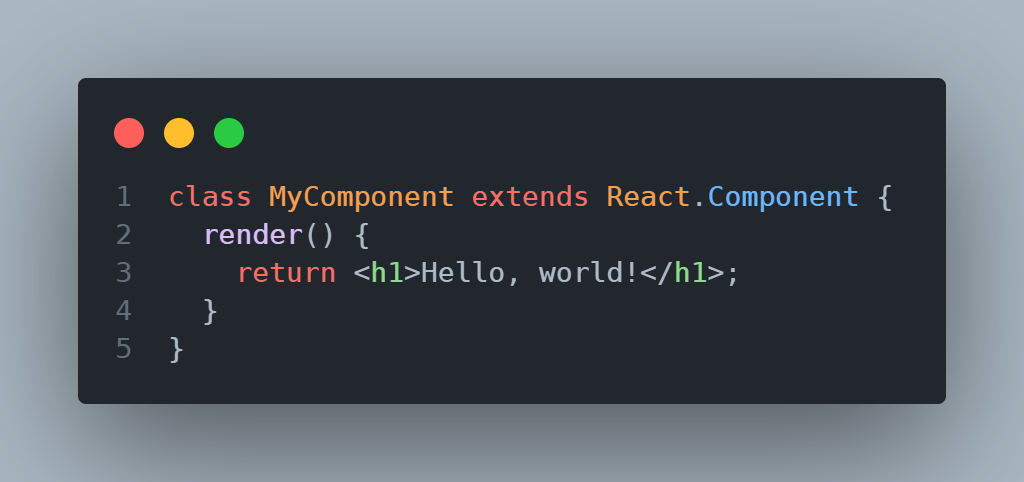
\includegraphics[width=100mm,scale=0.25]{myComponent.png}
\end{frame}

% Diapositiva 2: Componentes Funcionales
\begin{frame}[fragile]
  \frametitle{Componentes Funcionales}
  \begin{itemize}
    \item Más simples y fáciles de escribir.
    \item No tienen estado propio (antes de los Hooks).
  \end{itemize}
    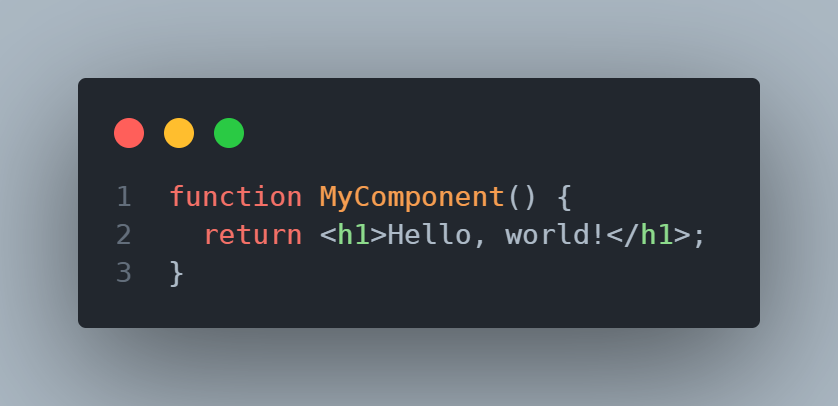
\includegraphics[width=75mm,scale=0.25]{myComponentFunction.png}
\end{frame}

% Sección 3: Props y Estado
\section{Props y Estado}

% Diapositiva 1: Props
\begin{frame}[fragile]
  \frametitle{Props}
  \begin{itemize}
    \item Los `props` son entradas que los componentes reciben de sus padres.
    \item Permiten pasar datos a los componentes hijos.
  \end{itemize}
    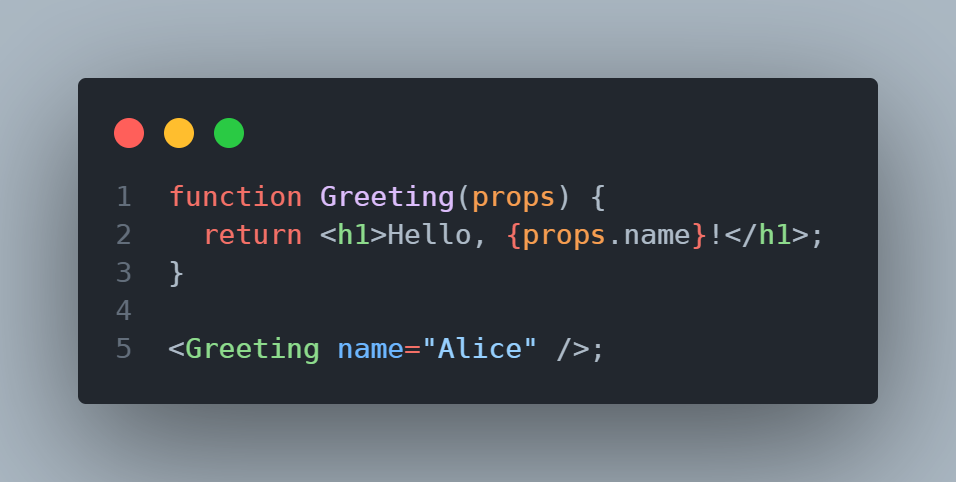
\includegraphics[width=100mm,scale=0.25]{03-props.png}

\end{frame}

% Diapositiva 2: Estado
\begin{frame}[fragile]
  \frametitle{Estado}
  \begin{itemize}
    \item El estado es un objeto privado del componente.
    \item Permite a los componentes gestionar y responder a cambios de datos.
  \end{itemize}
    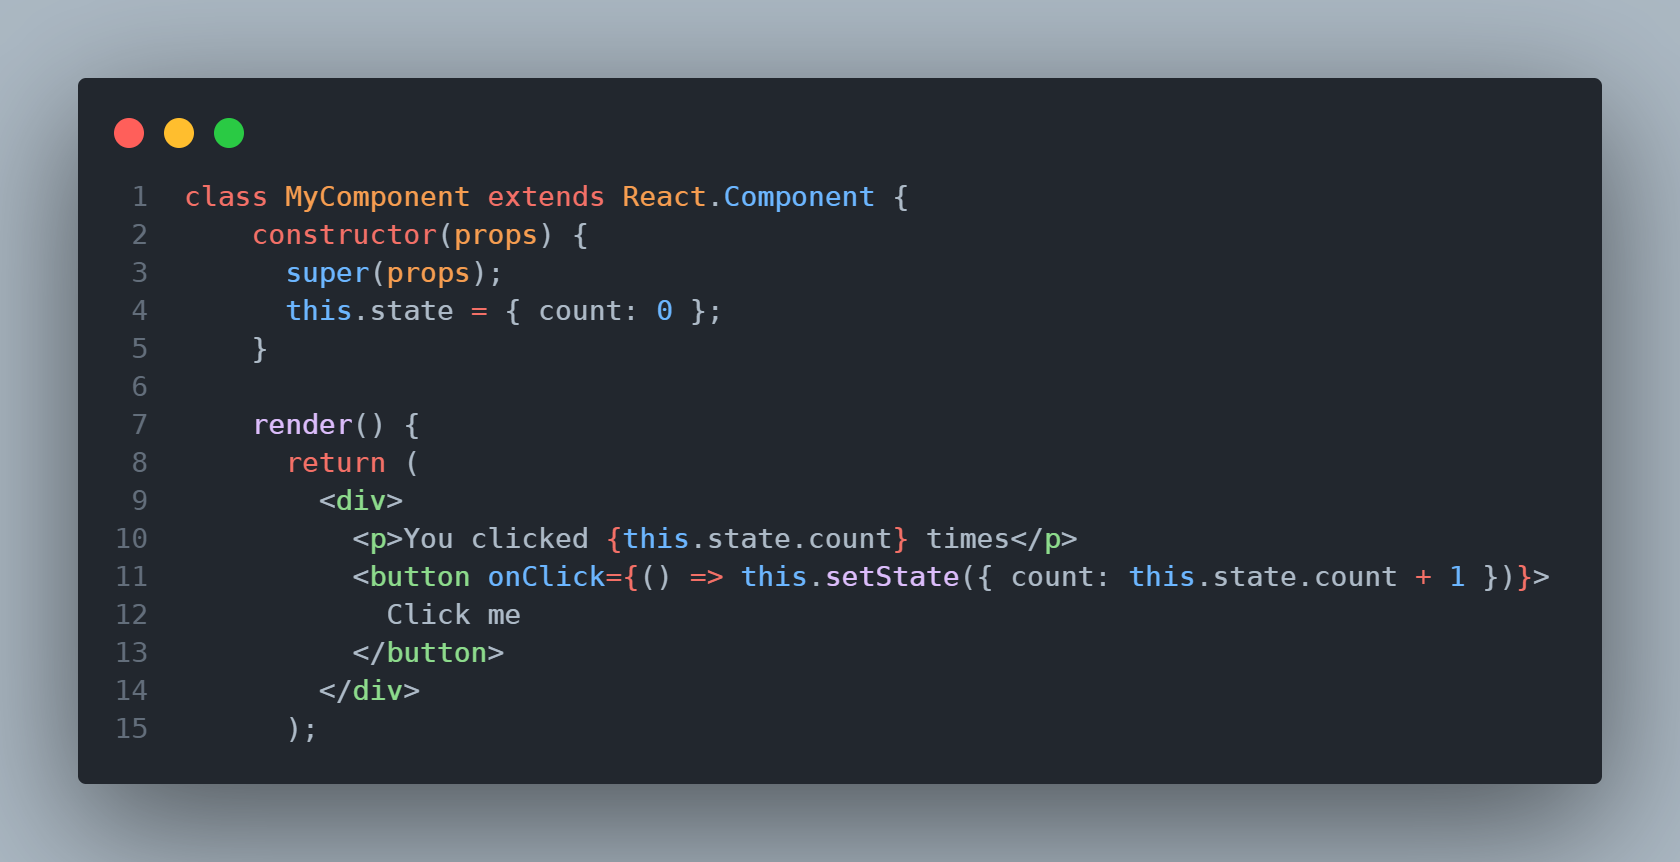
\includegraphics[width=110mm,scale=0.25]{04-estado.png}
\end{frame}

% Sección 4: Ciclo de Vida de los Componentes
\section{Ciclo de Vida de los Componentes}

% Diapositiva 1: Métodos del Ciclo de Vida
\begin{frame}
  \frametitle{Métodos del Ciclo de Vida}
  \begin{itemize}
    \item `componentDidMount`
    \item `componentDidUpdate`
    \item `componentWillUnmount`
  \end{itemize}
  \pause
  \begin{itemize}
    \item Permiten ejecutar código en diferentes etapas del ciclo de vida del componente.
  \end{itemize}
\end{frame}

% Diapositiva 2: Ejemplo de Método del Ciclo de Vida
\begin{frame}[fragile]
  \frametitle{Ejemplo de Método del Ciclo de Vida}
    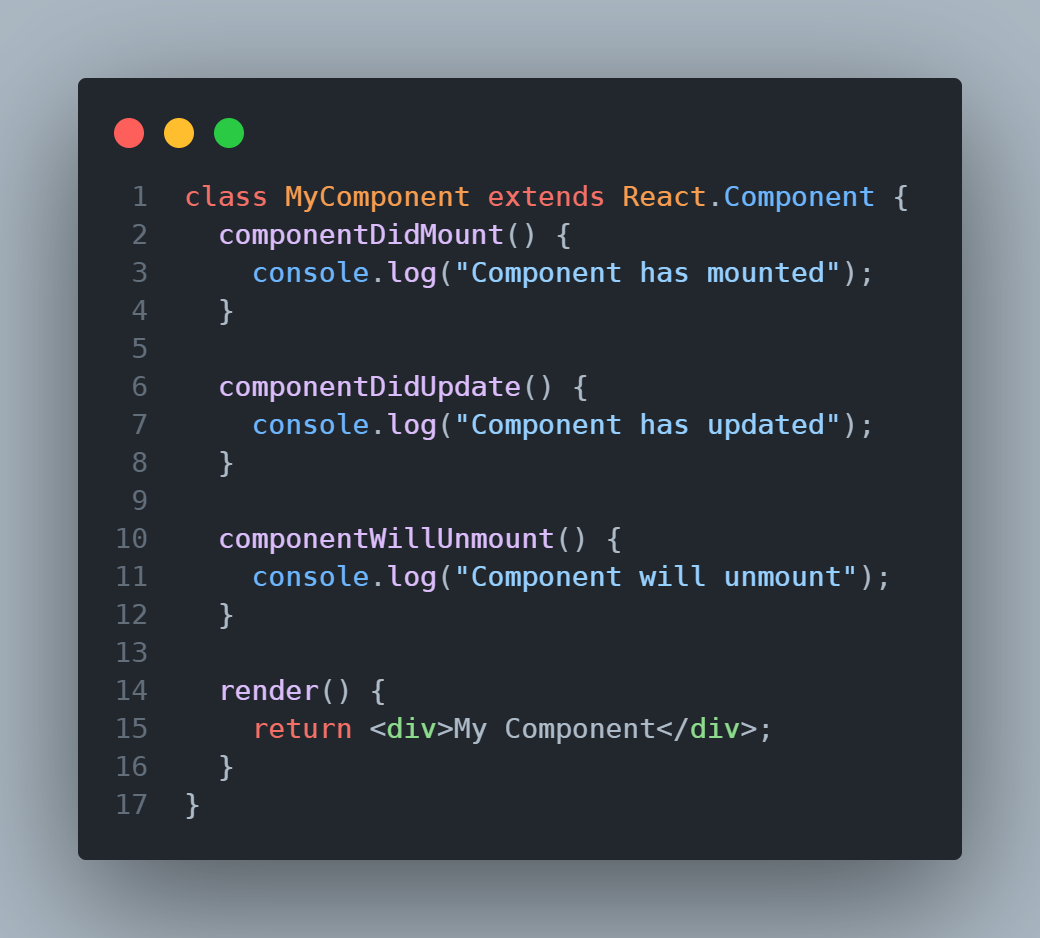
\includegraphics[width=90mm,scale=0.25]{05-cicloDeVida.png}
\end{frame}

% Diapositiva de resumen
\begin{frame}
  \frametitle{Resumen}
  \begin{itemize}
    \item React utiliza componentes para construir interfaces modulares.
    \item Los componentes pueden ser definidos como clases o funciones.
    \item Props y estado son fundamentales para la gestión de datos en React.
    \item Los métodos del ciclo de vida permiten manejar eventos en las diferentes etapas del componente.
  \end{itemize}
\end{frame}


\end{document}
